\documentclass[12pt,a4paper]{article}
\pagestyle{plain}
\usepackage{fullpage}
\usepackage[english]{babel}
\usepackage{enumerate}

%equations
\usepackage[fleqn]{amsmath}
\numberwithin{equation}{section}

%figures
\usepackage[dvips]{graphicx}
\graphicspath{{./images/}}
\numberwithin{figure}{section}

%excercises
\newcounter{Exercise}
\setcounter{Exercise}{1}
\usepackage[dvipsnames]{xcolor}
\usepackage{framed}
\definecolor{shadecolor}{gray}{0.9}
\usepackage{caption}

%tables
\numberwithin{table}{section}

%specials
\usepackage{textcomp} %special (greek) characters as text
%\usepackage{pstricks} %
%\usepackage{ifthen} %
%\usepackage{calc} %
%\usepackage{isotope}
\usepackage{hyperref}
\usepackage[bottom]{footmisc} %footnote below figure
\usepackage{footnpag}%number footnotes per page


%document details
\author{N.G. Schultheiss \\ translated and adapted by K. Schadenberg}
\date{}
\title{Solar Winds}


\begin{document}
\maketitle

\section{Introduction}
This module follows upon `The Sun' and can be continued by `Cosmic Radiation'.

\section{Solar Wind}
The Sun emits large amounts of electromagnetic radiation. But this is not the only thing it hurtles into space, it also `blows' large streams of charged particles into space.

The fusion processes taking place inside the Sun create different particles. We already saw a few of them in the previous module. We discussed photons as being electromagnetic radiation. Neutrinos are also created in vast amounts during the fusion process, these particles have no charge and are nearly (?) massless. As a consequence they leave the Sun almost unhindered.

Electrons and (to a lesser degree) positrons are also present in the Sun so we would expect to find them in the Solar winds. But because the positrons react readily with electrons we will not find many.

And then there are the charged atomic nuclei. Together with electrons they form the bulk of the Solar winds. Most are hydrogen nuclei, single protons, far fewer heavier ions are present.

Near the Earth the Solar wind has a density of roughly 10 particles per cubic metre. Most of these particles were emitted from one of two regions, the poles or Sunspots. Particles from the poles have an average speed of 400~km/s while the particles from the Sunspots move faster, nearly 800~km/s. 

\begin{shaded}
\textbf{Exercise \theExercise \stepcounter{Exercise}} : Lets assume that, at a certain time, there are only particles coming from the poles of the Sun (perhaps because the Sunspots are on the opposite side of the Sun). How many of these particles will flow through a surface of 1~m$^2$ every second?

You just calculated the flux of particles: the rate of flow per unit area. In this case, particles per second per metre squared.\end{shaded}

\section{Kinetic Energy}
We can measure the speed of particles inside the Solar wind in metres per second (m/s). Usually however, energy and not the speed of the particles is measured. Because we are talking about moving particles we are interested in the kinetic energy. According to classical (or Newtonian) physics the energy of a moving body, with a mass $m$ can be derived in the following manner:
\begin{align}
F \Delta t &= m \Delta v \\
F &= m \frac{\Delta v}{\Delta t}
\end{align}
If the force on the body is known we can calculate the work done by this force:
\begin{equation}
W = Fs = m \frac{\Delta v}{\Delta t} s
\end{equation}
Work is a form of energy transfer, this allows us to calculate the energy change of the body\footnote{To keep matters simple we assumed a constant force. What does this mean for the acceleration between $t_{\mbox{\begin{tiny}start\end{tiny}}}$ and $t_{\mbox{\begin{tiny}end\end{tiny}}}$?}:
\begin{align}
& s = v_{\mbox{\begin{tiny}average\end{tiny}}}\left( t_{\mbox{\begin{tiny}end\end{tiny}}} - t_{\mbox{\begin{tiny}start\end{tiny}}} \right) \\
& \Delta E = W = m \frac{v_{\mbox{\begin{tiny}end\end{tiny}}} - v_{\mbox{\begin{tiny}start\end{tiny}}}}{t_{\mbox{\begin{tiny}end\end{tiny}}} - t_{\mbox{\begin{tiny}start\end{tiny}}}} v_{\mbox{\begin{tiny}average\end{tiny}}}\left( t_{\mbox{\begin{tiny}end\end{tiny}}} - t_{\mbox{\begin{tiny}start\end{tiny}}} \right) \\
& E_{\mbox{\begin{tiny}end\end{tiny}}} - E_{\mbox{\begin{tiny}start\end{tiny}}} = m \left( v_{\mbox{\begin{tiny}end\end{tiny}}} - v_{\mbox{\begin{tiny}start\end{tiny}}} \right) \frac{v_{\mbox{\begin{tiny}start\end{tiny}}} + v_{\mbox{\begin{tiny}end\end{tiny}}}}{2}
\end{align}
We take $E_{\mbox{\begin{tiny}start\end{tiny}}}=0$~J and $v_{\mbox{\begin{tiny}start\end{tiny}}}=0$~m/s :
\begin{equation}
E_{\mbox{\begin{tiny}end\end{tiny}}} = m v_{\mbox{\begin{tiny}end\end{tiny}}} \frac{v_{\mbox{\begin{tiny}end\end{tiny}}}}{2}
\end{equation}
Generalising this equations yields:
\begin{equation}
E=\frac{1}{2}mv^2 \label{eq:Ekin}
\end{equation}

\begin{shaded}
\textbf{Exercise \theExercise \stepcounter{Exercise}} : Calculate the kinetic energy of a proton, with mass $1.67262158 \cdot 10^{-27}$~kg, travelling at a speed of 400~km/s.\end{shaded}

\begin{shaded}
\textbf{Exercise \theExercise \stepcounter{Exercise}} : What is the unit of energy when calculated using equation~\ref{eq:Ekin}?\end{shaded}

In most cases energy is expressed in Joules, J. But the kinetic energy of a single proton, even when travelling very fast, is only a fraction of one Joule. In this situation it is therefore more convenient to choose a smaller measurement of energy. In particle physics the electron volt, eV, is the unit of choice. The volt has a very specific definition, but one way of looking at it is the amount of (electrical) energy per unit charge:
\begin{equation}\begin{aligned}
& 1\mbox{V} = \frac{1\mbox{J}}{1\mbox{C}} \\
& 1\mbox{V} \cdot 1\mbox{C} = 1\mbox{J}
\end{aligned}\end{equation}

The elementary charge, the charge of a single proton, is e~$= 1.60217646 \cdot 10^{-19}$~C. This means:
\begin{equation}
1\mbox{eV}=1.60217646 \cdot 10^{-19} \mbox{C} \cdot 1\mbox{V} = 1.60217646 \cdot 10^{-19}\mbox{J}
\end{equation}

\begin{shaded}
\textbf{Exercise \theExercise \stepcounter{Exercise}} : Convert the answer of the previous exercise into our new unit, the electron volt.\end{shaded}

\section{Magnetic Fields}
\subsection{Charges in a magnetic fields}
A moving charge is an electric current. When a charge moves inside a magnetic field it will experience a force parallel to both the direction of travel and the magnetic field lines. This force is called the magnetic force.\footnote{Sometimes this is referred to as the Lorentz force. This is partly true. The Lorentz force is the force exerted by an electromagnetic field on a charged particle. It has two parts, the electric force and magnetic force.} You may have seen this force described as the force on a wire inside a magnetic field:
\begin{equation*}
F=BIL \hspace{10 mm} \mbox{or} \hspace{10 mm} F=BIL \sin \theta
\end{equation*}
A more formal way of writing this is as follows:
\begin{equation}
\mathbf{F}=\mathbf{I}L \times \mathbf{B} \label{eg:lorentz_wire}
\end{equation}
The force $\mathbf{F}$, electrical current $\mathbf{I}$, and magnetic field strength $\mathbf{B}$ are printed with bold letters. This is because these quantities are \textit{vectors}, they have a magnitude and direction. The product of the two terms is a special product, the cross (or vector) product. The result of this calculation depends on the angle between the two, as is the case in the less formal notation. 

For a single charged particle equation~\ref{eg:lorentz_wire} changes into:
\begin{equation}
\mathbf{F}=q\mathbf{v \times B} \label{eq:lorentz}
\end{equation}
$\mathbf{v}$ is the velocity (speed with direction) of the particle which has a charge $q$.\footnote{In other text the capital Q is sometimes used.}

What does this mean for particles moving inside a magnetic field? Take a look at figure~\ref{fig:lorentz}. A particle with no charge ($q=0$) is not deflected by the field. Particles with opposite charges are deflected in opposite directions. The direction of the force (and therefore deflection) follows from the cross product. A useful mnemonic that can be used to visualise the direction of the force is the right hand rule. The right hand rule can be explained in two different ways:
\begin{figure}\begin{center}
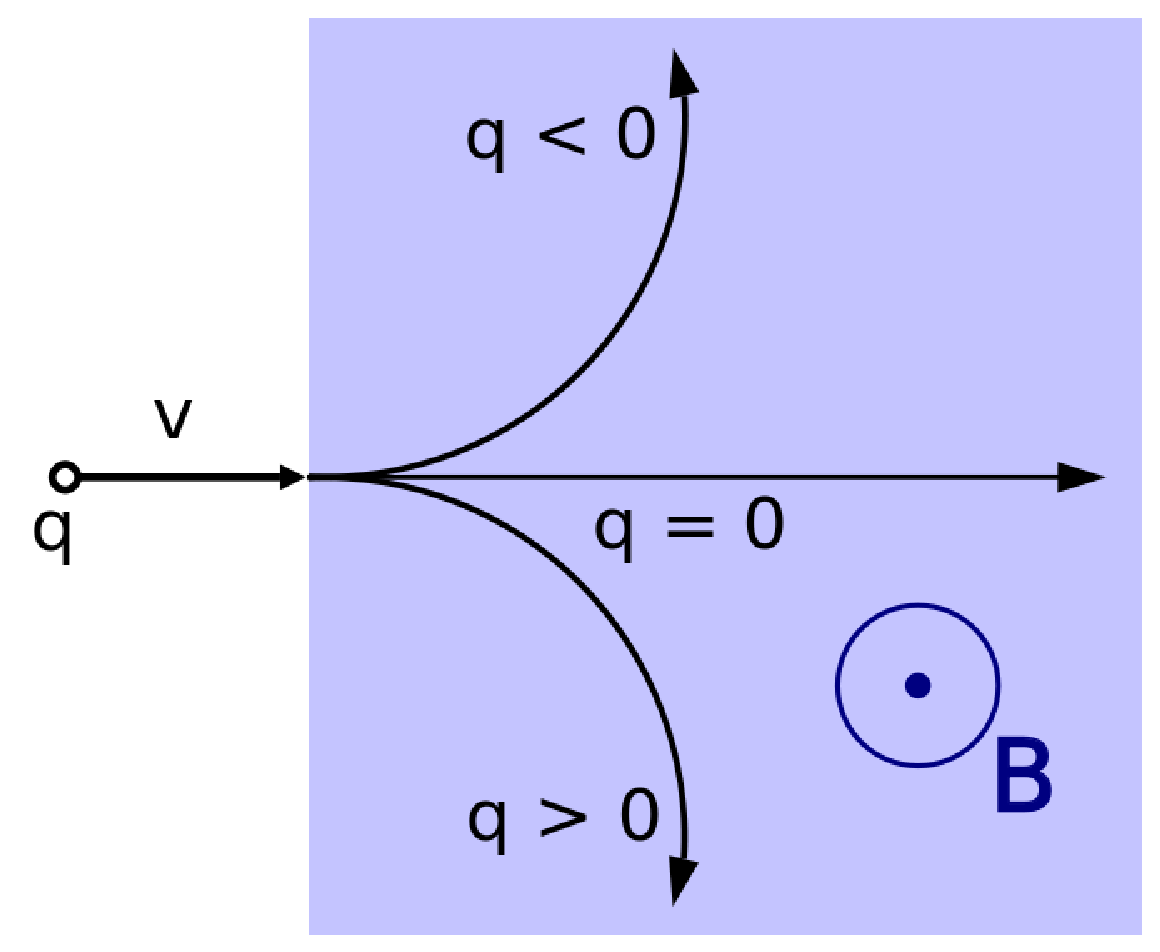
\includegraphics[scale=0.5]{Lorentz_force.svg.eps}%
\caption{The path of differently charged particles inside a magnetic field. The direction of the field is indicated by the dot; perpendicularly out of the paper.} \label{fig:lorentz}
\end{center}\end{figure}
\begin{itemize}
\item Use your right hand, point your fingers in the direction of the magnetic field and your thumb into the direction of the velocity. The palm of your hand now points into the direction of the force.
\item Curl the fingers of your right hand as if rotating the velocity vector $\mathbf{v}$ towards the direction of the magnetic field lines. Your thumb now points towards the direction of the force.
\end{itemize}
With both techniques take care to notice the sign of the charge. An electron has a charge of minus one, this effectively reverses the direction of travel (of the current).

\begin{shaded}
\textbf{Exercise \theExercise \stepcounter{Exercise}} : What would be the shape of the path of the charges in figure~\ref{fig:lorentz} if the magnetic field was much larger in size?\end{shaded}

The field of figure~\ref{fig:lorentz} is a uniform field, the strength and direction of the field is the same everywhere. Lets take a look at a slightly more complicated field: a divergent field. In figure~\ref{fig:lorentz_div} three field lines are drawn which clearly do not run parallel to each other. In the same figure the path of a single charge is drawn. At $v_1$ we start to follow the path of the particle. Its direction of travel is almost parallel to the field lines. At $v_2$ we determine the influence of the field on the particle. Using vector decomposition we can split the velocity of the particle into two parts; one which is parallel to the magnetic field and one which is perpendicular to the field. Only the perpendicular part will `feel' the magnetic force. Using the right hand rule we find that the magnetic force is directed along the dotted circle. The particle will start to move slightly into the direction of this circle. Because there is also a forward motion the particle will start to move in path spiralling around the field lines.
\begin{figure}\begin{center}
\begin{picture}(0,0)%
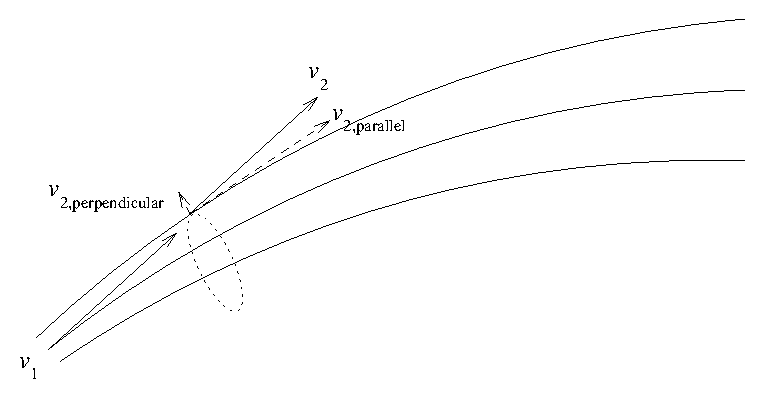
\includegraphics{lorentz}%
\end{picture}%
\setlength{\unitlength}{4144sp}%
%
\begingroup\makeatletter\ifx\SetFigFont\undefined%
\gdef\SetFigFont#1#2#3#4#5{%
  \reset@font\fontsize{#1}{#2pt}%
  \fontfamily{#3}\fontseries{#4}\fontshape{#5}%
  \selectfont}%
\fi\endgroup%
\begin{picture}(5558,2768)(391,-2641)
\end{picture}%
\caption{Lorentz forces in a divergent field.}\label{fig:lorentz_div}
\end{center}\end{figure}

\subsection{The Sun}
The Sun, like the Earth, has a magnetic field but much stronger. The magnetic field of the Sun is much more active and turbulent. In the past 2.000.000 years the magnetic field of the Earth has turned around seven times. In the Sun this happens every 7 to 15 years. Sun spots are regions of strong magnetic activity, but these spots are not always present. In their absence we only need to look at the poles of the Sun to determine the magnetic field.

Besides the magnetic force there is also an electrical force. Equal charges repel while opposites attract. The Sun emits large numbers of charged particles which will spiral along the magnetic field lines near the Sun. But at larger distances, roughly three times the radius of the Sun and larger, the electrical forces become to large to neglect. The particles no longer follow the magnetic field lines but start to move in the equatorial plane of the Sun. This heliospheric neutral sheet has an influence on the intensity of cosmic rays near the Earth (see figure~\ref{fig:sun_field}).  

\begin{figure}\begin{center}
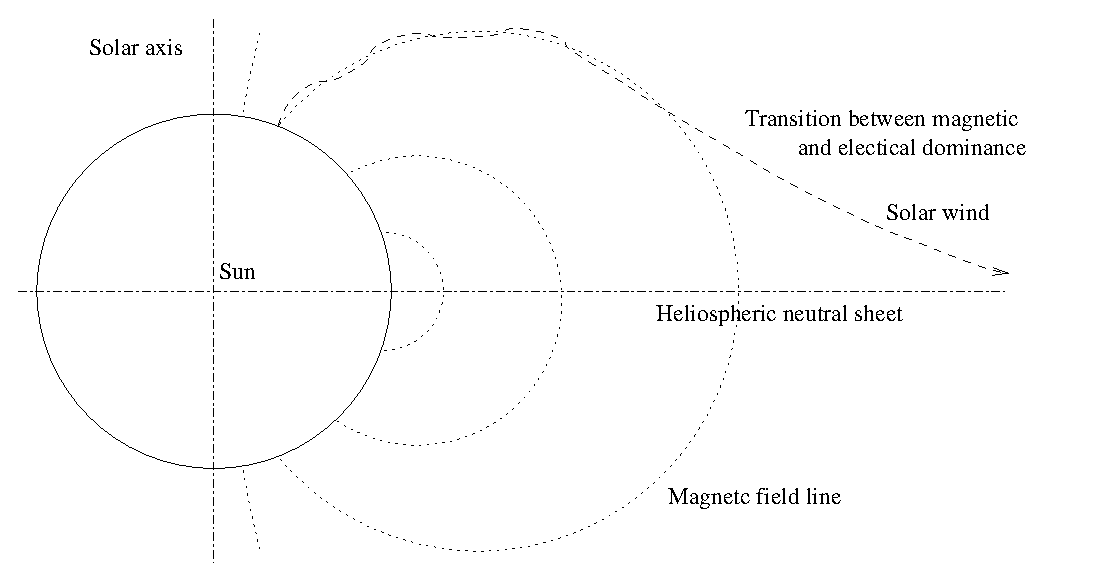
\includegraphics[scale=0.88]{orbit.eps}
\caption{The Solar winds near the Sun without Sun spots.} \label{fig:sun_field}
\end{center}\end{figure}

When there are Sun spots the magnetic field of the Sun becomes more complicated. Every spot is a magnetic pole. It frequently happens that a glowing hot stream of mass follows the field lines running from pole to pole, a Solar flare. Although very hot, this stream of mass is cooler than the photosphere, therefore a Sun spot below these flares appears darker than its surroundings.

\begin{shaded}
\textbf{Exercise \theExercise \stepcounter{Exercise}} : Because the Solar spots are so active they sling particles into space with more energy. The speed of these particles can be as large as 800~km/s. What is the energy, in eV, of these particles if they are protons?\end{shaded}

\subsection{The Earth}
The Earth is not alone in the universe, it constantly `feels' the magnetic field from the Sun and is exposed to the Solar winds. The lightest charged particles, the electrons, are captured first in the magnetic field of the Earth. They get trapped inside two large rings, the van Allen Belts. Heavier particles such as protons require a larger force to be deflected from their path. Most of the captured protons and heavier ions can be found in the inner van Allen belt.

Not all particles get trapped inside the van Allen belts, some are directed towards the poles. Here the magnetic field lines of the Earth converge. The strength of the field increases and because of the orientation of the field the particles are slowed down. When the particles reach the atmosphere they can collide with the atoms high up in the air. When they do, they light up the sky and forming Aurorae, in the Arctic region it is called the aurora borealis or northern lights. On the other side of the Earth, the same phenomenon is called the aurora australis, or southern lights.

Some particles have enough energy (are going fast enough) that the magnetic field of the Earth is unable to deflect them away from the Earth surface or towards poles. These particles, or the particles they create when they collide with atoms, can be observed with a detector placed on the surface of the Earth.

\end{document}
